\documentclass[12pt,letterpaper,noanswers]{exam}
%\usepackage{color}
\usepackage[usenames,dvipsnames,svgnames,table]{xcolor}
\usepackage[margin=0.9in]{geometry}
\renewcommand{\familydefault}{\sfdefault}
\usepackage{multicol}
\pagestyle{head}
\usepackage{hyperref}
\definecolor{c07}{HTML}{BBFFBB}
\definecolor{c08}{HTML}{BBFFFF}
\definecolor{c09}{HTML}{BBDDFF}
\definecolor{c10}{HTML}{BBBBFF}
\definecolor{c11}{HTML}{DDBBFF}
\definecolor{c12}{HTML}{BBBBDD}
\newcommand{\mb}[1]{\underline{#1}}

\header{AM 22b Problem Set 04}{}{Due Thurs Mar 4 at 6pm ET}
\runningheadrule
\headrule
\usepackage{diagbox}
\usepackage{graphicx} % more modern
%\usepackage{subfigure} 
\usepackage{amsmath} 
\usepackage{amssymb} 
%\usepackage{gensymb} 
%\usepackage{natbib}
\usepackage{hyperref}
%\usepackage{enumitem}
%\setlength{\parindent}{0pt}
%\usepackage{setspace}
%\pagestyle{empty}  
%\newcommand{\Sc}[0]{
%{\color{BlueViolet}\S}
%}
\usepackage{tcolorbox}

\begin{document}
 \pdfpageheight 11in 
  \pdfpagewidth 8.5in

\begin{questions}
\question Log in to WeBWorK and complete the problems assigned there under pset04.





\item For the following, identify whether the statement is true or false.  Include a justification of your choice.
\begin{parts}
\part If $f(x,y) = k$ for all points $(x,y)$ in a region $R$ then $\int_R f\ dA = k \cdot \text{Area}(R)$.
\begin{solution}
We have $\int_R k\ dA$ with $k$ a constant.  Since constants can come out of an integral, this is 
\[\int_R k\ dA = k\int_R dA = k\cdot \text{Area}(R).\]  The statement is true.
\end{solution}
\part If $R$ is the rectangle $0 \leq x \leq 1, 0 \leq y \leq 2$ and $S$ is the square $0\leq x \leq 1, 0 \leq y \leq 1$, then $\int_R f\ dA = 2\int_S f\ dA$.
\begin{solution}
This statement is sometimes true, so is false for the purposes of this problem.  Consider the function $f = x$.  $\int_R x\ dA > 2\int_S x\ dA$ because the function is smaller on $S$ than it is on the rest of $R$.
\end{solution}
% \part The iterated integrals \[\int_{-1}^1\int_0^1\int_0^{1-x^2}f\ dzdydx\] and \[\int_0^1\int_0^1\int_{-\sqrt{1-z}}^{\sqrt{1-z}}f\ dxdydz\] are equal.
% \begin{solution}
% The first region is given by $-1\leq x\leq 1$ and $0\leq y \leq 1$ and $0\leq z \leq 1-x^2$.  

% The second region has identical $y$ bounds (and the shapes do not vary with $y$).  This means we just need to compare whether the regions take up the same portion of the $xz$-plane.  

% In the $xz$-plane we are comparing $-1\leq x\leq 1$ and $0\leq z \leq 1-x^2$ to $0\leq z\leq 1$ and $-\sqrt{1-z}\leq x \leq \sqrt{1-z}$.

% The shape on the left is the region above $z = 0$ and below the parabola $z = 1-x^2$.  The constraints $-1\leq x\leq 1$ come from the intersection of $z=0$ and the parabola.

% The shape in the right is the region to the left of $-\sqrt{1-z} = x$, to the right of $x=\sqrt{1-z}$, and above $z=0$.  The left and right constraint curves both convert to $x^2 = 1-z \Rightarrow z = 1-x^2$.  So this is also the region above $z = 0$ and below the parabola $z= 1-x^2$.

% The region in the $xz$-plane is identical for both objects and the $y$-bounds match as well, so these integrals have the same region of integration.  They also have the same integrand, so the equality holds and the statement is true.
% \end{solution}

\end{parts}

\item Evaluating an integral example video: \url{https://www.youtube.com/watch?v=DgsTXYpbcu4}
\begin{parts}
\item Sketch the region of integration and evaluate the integral for \[\int_1^4\int_{\sqrt{y}}^y x^2y^3\ dx\ dy.\]

\begin{solution}
This region is $\sqrt{y}\leq x\leq y$ with $1\leq y\leq 4$.  So $x$ goes from $\sqrt{y}$ up to $y$:

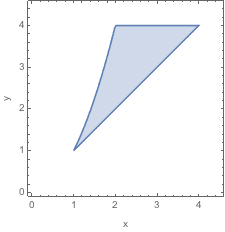
\includegraphics[width=2in]{img/HW06_r3.png}

\texttt{RegionPlot[1 <= y <= 4 \&\& Sqrt[y] <= x <= y, \{x, 0, 4.5\}, \{y, 0, 4.5\}, 
 FrameLabel -> \{"x", "y"\}]}
 
 To evaluate:
 \begin{align*}
 \int_1^4\int_{\sqrt{y}}^y x^2y^3\ dx dy = &\ \int_1^4\frac{1}{3}y^3\left.(x^3)\right\vert_{x=\sqrt{y}}^{x=y}\ dy\\
 =&\ \int_1^4\frac{1}{3}y^3(y^3-y^{3/2})\ dy \\
  =&\ \frac{1}{3}\int_1^4y^6-y^{9/2}\ dy \\
    =&\ \frac{1}{3}\left.(\frac{1}{7}y^7-\frac{2}{11}y^{11/2})\right\vert_1^4 \\
    =&\ \frac{1}{3}(\frac{1}{7}(4^7-1)-\frac{2}{11}(4^{11/2}-1)) \\
        =&\ \frac{1}{21}(4^7-1)-\frac{2}{33}(4^{11/2}-1) \\
 \end{align*}
\end{solution}

\item For the two regions shown below, compute the integral of $f(x,y) = xy$ over the region shown.

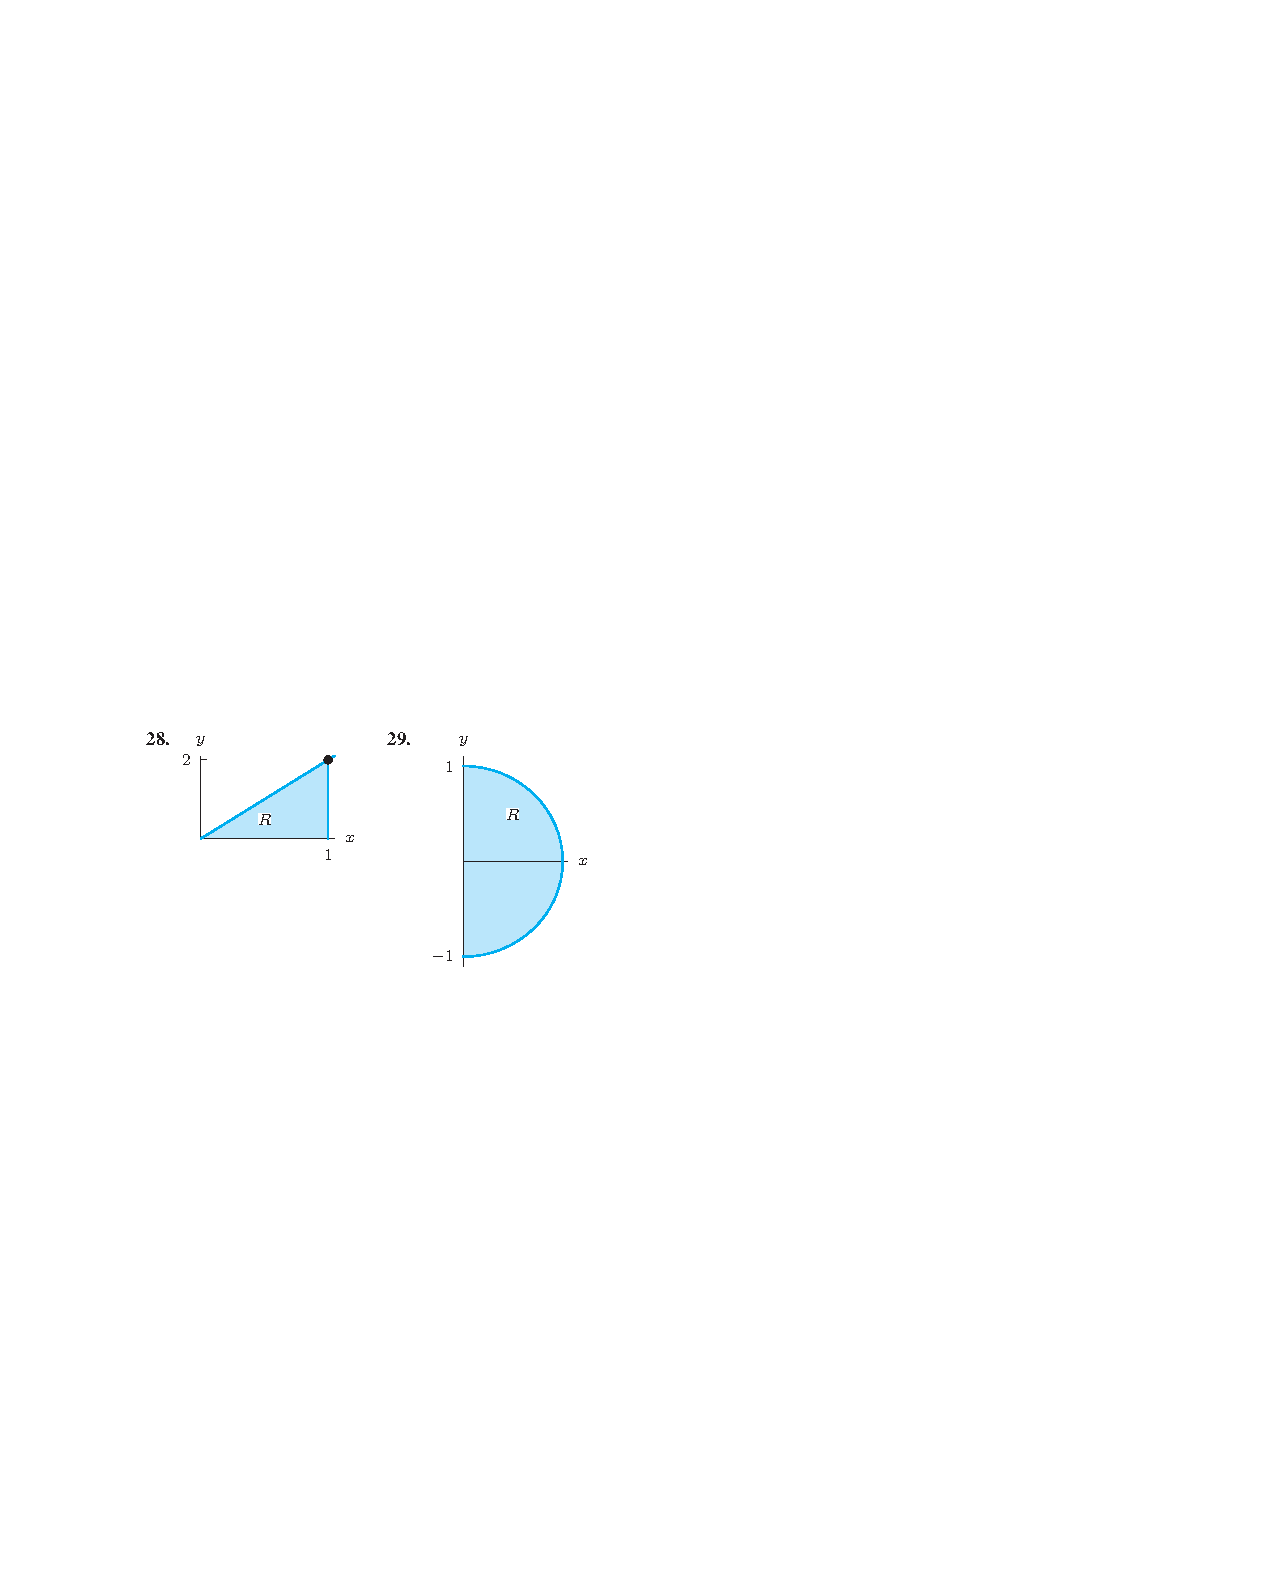
\includegraphics{img/HW06p1.pdf}

\begin{solution}
For the region on the left, we have $0\leq y\leq 2x$ since the bounding line goes from $(0,0)$ to $(1,2)$.  In addition, $0\leq x\leq 1$.  Setting up an integral, this is \begin{align*}
\int_0^1\int_0^{2x} xy\ dy\ dx &= \frac{1}{2}\int_0^1 x\left(\left.y^2\right\vert_0^{2x}\right)\ dx\\
&= \frac{1}{2}\int_0^1 x(4x^2)\ dx\\
&=2\int_0^1 x^3\ dx\\
&=2\frac{1}{4}\left.x^4\right\vert_0^1 \\
&= \frac{1}{2}.
\end{align*}

For the region on the right, we have a symmetry.  Specifically, at a fixed value of $x$, along a line through the object, we have $y<0$ below the $x$-axis and $y>0$ above the $x$-axis, with a symmetry in the shape of the object on either side of the axis.  The interior integral of $\int_0^1x\int_{-\sqrt{1-x^2}}^{\sqrt{1-x^2}} y\ dy\ dx$ is $0$ so the integral of $xy$ over the region will be zero.
\end{solution}

\end{parts}

% \item Log in to WeBWorK and complete the 7 problems assigned there under HW06.  \textbf{Write up WeBWorK problems 2, 3, 4, and 5 to be turned in as part of this assignment}.  WeBWorK will grade these for correctness.  In your write-up, they will be graded for your setup and showing the steps of working through the problem.  \emph{Note: You may need to review $u$-substitutions to complete some of the integrals.}
% \begin{parts}
% \item Webwork Q2
% \item Webwork Q3
% \item Webwork Q4
% \item Webwork Q5
% \end{parts}



\item Convert the following from polar coordinates to Cartesian coordinates or from Cartesian coordinates to polar coordinates.  Sketch each curve in the $xy$-plane.
\begin{parts}
\item $r=\frac{2}{\sin\theta}$.

\item $y=\sqrt{1-x^2}$.

\item $r=\frac{1}{\cos\theta}$.

\item $\theta = 3\pi/4$.

\end{parts}


\item Electric charge is distributed throughout $3$-space, with density proportional to the distance from the $xz$-plane.  Show that the total charge inside of a cylinder of radius $R$ and height $h$ that sits on the $xz$-plane and is centered along the $y$-axis is proportional to $R^2h^2$.  \emph{You may want to think about this using a ``cylindrical'' coordinate system centered about a different axis than usual.}

\question Suppose $W$ is the region outside the cylinder $x^2+y^2 = 1$ and inside the sphere $x^2+y^2+z^2 = 2$.  Calculate \[\int_W (x^2+y^2)\ dV.\]  Include a sketch of a cross-section of the region in the $rz$-half plane.

\question (Center of mass of a \emph{Tyrannosaurus rex})

This data is from the authors of \cite{hutchinson2011computational}.  We have permission to use it for the purposes of this activity only.  It is based on a lidar scan of a \emph{T. rex} skeleton.

The matlab data in \texttt{TRex.mat} is in pixels.  There are two sets of pixels: a lower resolution and a higher resolution set.  For all of your work on this problem, assume the top of the head of the \emph{T. rex} is at 4.7m for each dataset.
\begin{parts}
\item Make scatter plots of both data sets.  Rescale your data so that it is in meters, rather than pixels.  Submit the plots (include the code in your Canvas submission, but it does not need to go onto Gradescope).  Remember axis labels.  Using \texttt{axis equal} will help the dinosaur skeleton be in the correct proportions.
\item (center of mass) Look up center of mass in the index of our course text (p. 890 in the 6th edition).  After reading about center of mass, develop a procedure for estimating the center of mass of the dinosaur skeleton using the data provided.  Make an assumption of uniform density for the bones.

Describe your plan in words (you may use pseudocode or complete sentences).
\item Estimate the center of mass for the dinosaur skeleton based on the data that was provided.  Do this for each resolution of data.  Submit a screenshot of your code on Gradescope, as well as your final estimates.
\item (moment of inertia) Modify your algorithm to estimate the moment of inertia instead of the center of mass.  Submit analogous deliverables to part (c).
\item We have data about the skeleton of this dinosaur.  Consider how the center of mass of the actual dinosaur might differ from that of its skeleton.  Given the skeleton, how might you estimate the center of mass of the dinosaur?  Describe your ideas.  Identify at least three assumptions that you would be making.

\emph{There are many possible approaches and choices of assumptions.}

\item (Optional) If you'd like, you can attempt to estimate the location of the center of mass of the dinosaur.
\end{parts}

\end{questions}

\bibliographystyle{plain}
\bibliography{pset}

\end{document}
